\documentclass[12pt,a4paper]{article}
\usepackage[utf8]{inputenc}
\usepackage{polski}
\usepackage{graphicx}
\usepackage{wrapfig}

\begin{document}

\title{Diamond Problem}
\author{Grzegorz Kowalski\\\texttt{daneos@daneos.com}}
\date{\today}
\maketitle

\section{Opis problemu}
\textbf{Diamond problem} to sytuacja, w której klasa (A) dziedziczy po dwóch klasach (B i C), dziedziczących z kolejnej (D).
Tworzy to niejednoznaczność ponieważ jeżeli klasy B i C nadpisują tę samą metodę dziedziczoną z klasy D, a klasa A jej nie nadpisuje, to nie wiadomo z której z tych klas powinna odziedziczyć ją klasa A.\\
Problem ten jest możliwy do napotkania tylko w językach, które pozwalają na dziedziczenie z kilku klas na raz.\\
Nazwa \emph{diamond problem} jest nawiązaniem do kształtu diagramu dziedziczenia w takiej sytuacji.

\section{Przykład}
\begin{wrapfigure}{r}{0.4\textwidth}
	\begin{center}
		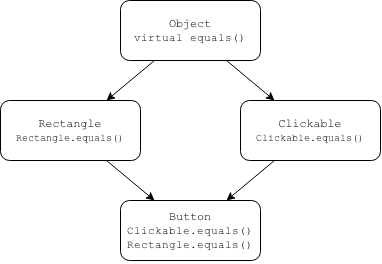
\includegraphics[scale=0.65]{diamond.png}
	\end{center}
\end{wrapfigure}
Klasa \texttt{Object} definiuje metodę \texttt{equals()}. Klasy \texttt{Rectangle} i \texttt{Clickable} dziedziczą po \texttt{Object} i nadpisują metodę \texttt{equals()} swoimi własnymi. Jesli klasa \texttt{Button} dziedziczy z \texttt{Rectangle} (wygląd) i \texttt{Clickable} (funkcjonalność), to wywołanie \texttt{Button.equals()} nie jest jednoznaczne.

\end{document}